%                                                                 aa.dem
% AA vers. 9.1, LaTeX class for Astronomy & Astrophysics
% demonstration file
%                                                       (c) EDP Sciences
%-----------------------------------------------------------------------
%
%\documentclass[referee]{aa} % for a referee version
%\documentclass[onecolumn]{aa} % for a paper on 1 column  
%\documentclass[longauth]{aa} % for the long lists of affiliations 
%\documentclass[letter]{aa} % for the letters 
%\documentclass[bibyear]{aa} % if the references are not structured 
%                              according to the author-year natbib style

%
\documentclass{aa}  

%
\usepackage{graphicx}
%%%%%%%%%%%%%%%%%%%%%%%%%%%%%%%%%%%%%%%%
\usepackage{txfonts}
%%%%%%%%%%%%%%%%%%%%%%%%%%%%%%%%%%%%%%%%
%\usepackage[options]{hyperref}
% To add links in your PDF file, use the package "hyperref"
% with options according to your LaTeX or PDFLaTeX drivers.
%
\begin{document} 
    

   \title{Cosmic Microwave Background Formation}


   \author{A. Wetzel
          }

   \institute{Department of Informatics - UiO\\
              \email{andrewet@ifi.uio.no}
             }

   \date{}

% \abstract{}{}{}{}{} 
% 5 {} token are mandatory
 
  % context heading (optional)
  % {} leave it empty if necessary  
  

   \keywords{Hubble parameter -- Conformal time -- Distance measures -- Free electron fraction --
                Optical depth --
                Visibility function
               }

   \maketitle
%
%-------------------------------------------------------------------
\section{Milestone 1}
\subsection{Introduction}
In this project we are going to look at the uniform background in the Universe and investigate the expansion history of the universe. We will do this by computing the expansion history of the universe numerical and analytical, and observe the uniform background densities for different components of matter and energy.  
\subsection{Theoretical background}
A uniform background universe describes the spatial distribution of matter to be homogeneous and isotropic observed at a large scale. This is also known as the Cosmological Principle. In this project we assume that the universe is flat which means that $k=0$ in the Friedmann–Lemaître–Robertson–Walker metric (FRLW)
\begin{align}
    ds^2 =-dt^2+a(t)^2(dx^2+dy^2+dz^2)\label{FLRW_cart}
\end{align}
Where equation \eqref{FLRW_cart} is in Cartesian coordinates. $a(t)$ is the only free variable in equation \eqref{FLRW_cart}, and it tells us how fast the Universe expands and how object behaves. To be able to evaluate the expansion of the Universe, we have to insert the metric \eqref{FLRW_cart} into the Friedmann equation, which is given in equation \eqref{eq:Friedmann_eq}
\begin{align}
    H=H_0\sqrt{(\Omega_{b0}+\Omega_{\text{CDM}0})a^{-3}+(\Omega_{\gamma0}+\Omega_{\nu0})a^{-4}\Omega_{k0}a^{-2}+\Omega_{\Lambda0}} \label{eq:Friedmann_eq}
\end{align}
for simplicity we say that $\Omega_{m0}=(\Omega_{b0}+\Omega_{\text{CDM}0})$ and $\Omega_{r0}=(\Omega_{\gamma0}+\Omega_{\nu0})$, further we
have the Hubble parameter, $H=\frac{da}{dt}\frac{1}{a}=\frac{\Dot{a}}{a}$ and the $\Omega$-values, which describes the relative densities for present day. $\Omega_{b0}\approx 0.05$ is for baryonic matter, $\Omega_{\text{CDM}0}\approx 0.25$ is for dark matter, $\Omega_{\gamma0}$ is for radiation, $\Omega_{\nu0}$ is for the neutrino energy and $\Omega_{\Lambda 0}\approx 0.7$ is for dark energy. The $\Omega_{k0}=-\frac{kc^2}{H_0^2}$ term describes the curvature, by setting $a=1$ we have that $\Omega_{k0}=1-\Omega_{m0}-\Omega_{r0}-\Omega_{\Lambda0}$. Since we don't include curvature we set $\Omega_{k0}=0$. 
Further we have that the radiation parameter and the neutrino energy is given as 
\begin{align}
    \Omega_{\gamma0}&= 2\cdot \frac{\pi^2}{30}\frac{(k_bT_{\text{CDM}0})^4}{\hbar^3c^5}\frac{8\pi G}{3H_0^2}\\
    \Omega_{\nu0}&=N_\text{eff}\cdot\frac{7}{8}\bigg(\frac{4}{11}\bigg)^\frac{4}{3}\Omega_{\gamma0}
\end{align}
where $T_{\text{CDM}0}=2.7255$K is today's temperature of the CMB, and $N_\text{eff}=3.0466$ is the effective number of neutrinos. \\
All these components and equation \eqref{eq:Friedmann_eq} is known as the standard model of cosmology.\\   
\\
We can also write the Friedmann equation on the following form
\begin{align}
    H=H_0=\sqrt{\frac{\rho_x}{\rho_c}} \label{eq:H_rho}
\end{align}
where $\frac{\rho_x}{\rho_c}=\Omega_{m0}+\Omega_{r0}+\Omega_{k0}+\Omega_{\Lambda 0}$ and $\rho_c=3H^2/(8\pi G)$.\\
The Friedmann equation can show us how each density components changes with time, this is given by the following equation
\begin{align}
    \Dot{\rho}+3H(\rho+P)=0
\end{align}
where $\rho$ is the density and $P$ is the pressure. This equation tells us how the components evolves over time. There is also the equation of state which is given as

    $\omega=\frac{P}{\rho}$ and $\omega$ will be constant.
Hence we have that 
\begin{align}
    \rho\propto a^{-3(1+\omega)}
\end{align}
Where
\begin{equation}
\omega=
\systeme{
  0\;\;\;\; \text{for cold dark matter and baryons},
  1/3\;\;\;\; \text{for radiation} \;\;\;\;\;\;\;\;\;\;\;\;\;\;\;\;\;\;\;\;\;\;\;\;\;\;\;\;\;,
  -1\;\;\;\; \text{for dark energy}\;\;\;\;\;\;\;\;\;\;\;\;\;\;\;\;\;\;\;\;\;\;\;\;\;
} \label{eq:omega_val}
\end{equation}
\\
\\
When we look at the cosmic microwave background, CMB, it is important to look at the \emph{comoving horizon}. Comoving horizon tells us how far the light has travelled after the Big Bang, where $t=0$. The comoving horizons expands with time, which we call \emph{conformal time}, $\eta$. We can write the conformal time in the following form
\begin{align}
    \frac{d\eta}{dt}&=\frac{c}{a}\label{eq:deta_t}\\
    &=\frac{d\eta}{da}\frac{da}{dt}\\
    &=\frac{d\eta}{da}aH \label{eq:deta_a}
\end{align}
We are now able to write $\eta$ as a function $x$ by using equation \eqref{eq:deta_t} and \eqref{eq:deta_a}
\begin{align}
    \frac{d\eta}{da}&=\frac{c}{a^2H}=\frac{c}{a\mathcal{H}}\\
    \frac{d\eta}{dx}&=\frac{da}{dx}\frac{d\eta}{da}=\frac{c}{\mathcal{H}}\\
    \eta(x)&=\int_{-\infty}^x\frac{cdx'}{\mathcal{H}(x')} \label{eq:eta_x}
\end{align}
where $\mathcal{H}=aH$ is a scaled version of the Hubble parameter.
\begin{align}
    \mathcal{H}=aH_0\sqrt{\Omega_{m0}a^{-3}+\Omega_{r0}a^{-4}\Omega_{k0}a^{-2}+\Omega_{\Lambda0}} \label{eq:Friedmann_eq_Hp}
\end{align}
There are several ways to measure the time in our Universe. One of these is the relation between time and scale factor. They have a one-to-one relation, which means we can use the scale factor to calculate the time.\\
 Another way to calculate time is to use the redshift, which is done by measuring the time by observing how far the wavelength of a photon has been extended after it was sent out at a time $t$.
\\
There are other ways to calculate the distances in the Universe as well. The calculations on the distances depends on the geometry.
 We are only going to look at the measurement on a flat universe, and one of the methods to calculate the distance is called \emph{comoving distance}. It excludes the expansion of then universe. Due to the expansion of space will a given distance not change over time. And with a given redshift $z$ can we write the comoving distance as
\begin{align}
    \chi &=\int_1^a\frac{cda}{a^2H}=\int_0^z\frac{cdz}{H}\\
    &=\eta-\eta_0
\end{align}
where
\begin{align}
    \chi=\int_t^{t_\text{today}}\frac{cdt}{a}=r
\end{align}
and $\frac{cdt}{a}=dr$ if a photon moves radially to us in a flat universe.
\\
There is also distance measure that is called \emph{angular distance measure}. This is a distance that is defined at the size, $\Delta s$, of an object with a given redshift which has an angular size $\Delta \theta$. It can be written in the following form
\begin{align}
    d_A=\frac{\Delta s}{\Delta \theta}=\frac{S_k(r)}{1+z}
\end{align}
where $S_k(r)=\chi$.\\
Another distance measure is the luminosity distance, this distance can be calculated by finding the flux, $F$, and the luminosity, $L$, and is given as
\begin{align}
    d_L=\sqrt{\frac{L}{4\pi F}}
\end{align}
we know the that $L\propto \frac{1}{a^4}$ and $F\propto\frac{1}{d_A^2}$, and we can therefore see a relation between luminosity distance and angular distance 
\begin{align}
    d_L&=\sqrt{\frac{1/a^4}{1/d_A^2}}\\
    &=\frac{d_A}{a^2}
\end{align}

\subsection{Method}
By calculating expansion history of the universe numerical we us a model which contains the cosmological parameters and functions which will give use the conformal time, distance measure and the Hubble parameter. As our time variable we will use the scale factor $a=e^{x}$.   
\\
We will compute and make plots of $H(x)$, $\mathcal{H}(x)$, $\frac{1}{\mathcal{H}(x)}\frac{d\mathcal{H}(x)}{dx}$, $\frac{1}{\mathcal{H}(x)}\frac{d^2\mathcal{H}(x)}{dx^2}$, $\eta(x)$, $\frac{\eta(x) is \mathcal{H}(x)}{c}$, $t(x)$, $\Omega_m$, $\Omega_r$ and $\Omega_\Lambda$, we use different functions for all the $\Omega$-values, which you can see below. 
\begin{align}
    \Omega_{k}(a)&=\frac{\Omega_{k0}}{a^2H(a)^2/H_0^2} \label{eq:Omega_k}\\
    \Omega_{\text{CDM}}(a)&=\frac{\Omega_{\text{CDM}0}}{a^2H(a)^2/H_0^2} \label{eq:Omega_CDM}\\
    \Omega_{b}(a)&=\frac{\Omega_{n0}}{a^3H(a)^2/H_0^2} \label{eq:Omega_b}\\
    \Omega_{\gamma}(a)&=\frac{\Omega_{\gamma0}}{a^4H(a)^2/H_0^2} \label{eq:Omega_gamma}\\
    \Omega_{\nu}(a)&=\frac{\Omega_{\nu0}}{a^4H(a)^2/H_0^2} \label{eq:Omega_nu}\\
    \Omega_{\Lambda}(a)&=\frac{\Omega_{\Lambda0}}{a^4H(a)^2/H_0^2} \label{eq:Omega_lambda}
\end{align}
\subsubsection{Position, redshift and time }
First of all we want calculate the times - $x$, $z$, $t$ for radiation-matter equality, matter-dark energy equality and when the Universe starts to accelerate. We will use these values to mark the transitions between the different phases and see how this effects the universe in different settings.\\
We start to compute the time for radiation-matter equality, $\Omega_{m}=\Omega_{r}$. We now that $\Omega_{m0}\propto a^{-3}$ and $\Omega_{r0}\propto a^{-4}$ we then get the equation
\begin{align}
    a^{-3}\Omega_{m0}&=a^{-4}\Omega_{r0}\\
    a_{MR}&=\frac{\Omega_{r0}}{\Omega_{m0}} \label{eq:a_MR}
\end{align}
Further we compute the time for matter-dark energy equality, $\Omega_{m}=\Omega_{\Lambda}$, and we have that $\Omega_{\Lambda}\propto 1$, which gives us
\begin{align}
    a^{-3}\Omega_{m0}&=\Omega_{\Lambda0}\\
    a_{MDE}&=\bigg(\frac{\Omega_{m0}}{\Omega_{\Lambda0}}\bigg)^{\frac{1}{3}} \label{eq:a_mde}
\end{align}
Finally we compute when the Universe starts to accelerate. We have that 
\begin{align}
    \Dot{a}=aH&=\sqrt{\Omega_{m0}a^{-3}+\Omega_{\Lambda0}}\\
    &=H_0\sqrt{\Omega_{m0}a^{-1}+\Omega_{\Lambda0} a^2}
\end{align}
This gives us now 
\begin{align}
    \Ddot{a}&=H_0\frac{1}{2}\frac{1}{\sqrt{\Omega_{m0}a^{-1}+\Omega_{\Lambda0} a^2}}\bigg(\Omega_{m0}\bigg(-\frac{1}{a^2}\bigg)\Dot{a}+2\Omega_{\Lambda0} a\Dot{a}\bigg)=0
\end{align}
We simplify this expression by cancelling out some values. This gives us
\begin{align}
    \Ddot{a}=\bigg(-\Omega_{m0}\frac{\Dot{a}}{a^2}+2\Omega_{\Lambda0} a\Dot{a}\bigg)&=0\\
    -\Omega_{m0}\frac{1}{a^2}+2\Omega_\Lambda a&=0\\
    2\Omega_{\Lambda0} a&=\Omega_{m0}\frac{1}{a^2}\\
    a&=\bigg(\frac{\Omega_{m0}}{\Omega_{\Lambda0}}\bigg)^\frac{1}{3} \label{eq:a_acc}
\end{align}
\\
We now insert equation \eqref{eq:a_MR}, \eqref{eq:a_mde} and \eqref{eq:a_acc} into equation \eqref{eq:x}-\eqref{eq:t} which will then gives us the different values for position, redshift and time for radiation-matter equality, matter-dark energy equality and when the Universe starts to accelerate.
\begin{align}
    x=\ln{a} \label{eq:x}\\
    z = \frac{1}{a}-1 \label{eq:z}\\
    t=t(\ln{a}) \label{eq:t}
\end{align}
\subsubsection{$H$ and $\mathcal{H}$}
We will now compute $H$, so we use equation \eqref{eq:Friedmann_eq} which is written as 
\begin{align}
     H(x)=H_0\sqrt{\Omega_{m0}e^{-3x}+\Omega_{r0}e^{-4x}\Omega_{k0}e^{-2x}+\Omega_{\Lambda0}} \label{eq:H_x}
\end{align}
as a function of x.\\
We insert equation \eqref{eq:Omega_k}-\eqref{eq:Omega_lambda} into equation \eqref{eq:H_x}.\\
To compute $\mathcal{H}$ we use equation \eqref{eq:Hp_eq}  
\begin{align}
    \mathcal{H}(x)&=e^xH_0\sqrt{{\Omega_{m0}e^{-3x}+\Omega_{r0}e^{-4x}\Omega_{k0}e^{-2x}+\Omega_{\Lambda0}}}\\
    &=H_0\sqrt{\Omega_{m0}e^{-x}+\Omega_{r0}e^{-2x}+\Omega_{k0}+\Omega_{\Lambda0}e^{2x}}\label{eq:Hp_eq}
\end{align}
and we will say that $$\Omega_{v1}=\Omega_{m0}e^{-x}+\Omega_{r0}e^{-2x}+\Omega_{k0}+\Omega_{\Lambda0}e^{2x}$$ which gives us \begin{align}
     \mathcal{H}(x)=H_0\sqrt{\Omega_{v1}} \label{eq:Hp_x_omega}
\end{align}  
\subsubsection{$\frac{1}{\mathcal{H}(x)}\frac{d\mathcal{H}(x)}{dx}$ and $\frac{1}{\mathcal{H}(x)}\frac{d^2\mathcal{H}(x)}{dx^2}$}
I chose to solve $\frac{1}{\mathcal{H}(x)}\frac{d\mathcal{H}(x)}{dx}$ and $\frac{1}{\mathcal{H}(x)}\frac{d^2\mathcal{H}(x)}{dx^2}$ analytically, and we therefore start to use derivation on equation \eqref{eq:Hp_x_omega}
\begin{align}
    \frac{d\mathcal{H}(x)}{dx}&=H_0\frac{1}{2}\frac{1}{\sqrt{\Omega_{v1}}}\Omega_{v1}'\\
    &=H_0\frac{1}{\sqrt{\Omega_{v1}}}(-\Omega_{m0}e^{-x}-2\Omega_{r0}e^{-2x}+\Omega_{k0}+2\Omega_{\Lambda0}e^{2x})\\
    &=H_0\frac{1}{2}\frac{1}{\sqrt{\Omega_{v1}}}\Omega_{v2} \label{eq:dHp_dx}
\end{align}
where $$\Omega_{v2}=(-\Omega_{m0}e^{-x}-2\Omega_{r0}e^{-2x}+\Omega_{k0}+2\Omega_{\Lambda0}e^{2x})$$\\
We are now able to calculate $\frac{1}{\mathcal{H}(x)}\frac{d^2\mathcal{H}(x)}{dx^2}$ by finding the derivative of equation \eqref{eq:dHp_dx}.
\begin{align}
   \frac{d^2\mathcal{H}(x)}{dx^2}&=\frac{1}{2}H_0(\Omega_{v2}'\Omega_{v1}^{-1/2}+\Omega_{v2}(\Omega_{v2}^{-1/2})' )\\
   &=\frac{1}{2}H_0\bigg(\frac{\Omega_{m0}e^{-x}+4\Omega_{r0}e^{-2x}+\Omega_{k0}+4\Omega_{\Lambda0}e^{2x}}{\Omega_{v1}}\nonumber\\&+\Omega_{v2}\bigg(-\frac{1}{2}\frac{1}{\Omega_{v1}^{3/2}}\Omega_{v1}'\bigg)\bigg)
\end{align}
we now say that $$\Omega_{v3}=\Omega_{m0}e^{-x}+4\Omega_{r0}e^{-2x}+\Omega_{k0}+4\Omega_{\Lambda0}e^{2x}$$ 
This will then give us
\begin{align}
    \frac{d^2\mathcal{H}(x)}{dx^2}&=\frac{1}{2}H_0\bigg(\frac{\Omega_{v3}}{\sqrt{\Omega_{v1}}}-\frac{1}{2}\frac{\Omega_{v2}}{{\Omega_{v1}^{3/2}}}\Omega_{v2}\bigg)\\
    &=\frac{1}{2}H_0\frac{1}{\sqrt{\Omega_{v1}}}\bigg(\Omega_{v3}-\frac{1}{2}\frac{\Omega_{v2}^2}{\Omega_{v1}}\bigg)
\end{align}
We have now found values for $\frac{d\mathcal{H}(x)}{dx}$ and $\frac{d^2\mathcal{H}(x)}{dx^2}$ analytically and we now insert these values into two function and dived each of them with $\mathcal{H}(x)$.\\
\subsubsection{$\eta(x)$ and $t(x)$}
To compute $\eta(x)$ and $t(x)$ we use the 4th-Order Runge Kutta for solving our ODEs. After we solved the ODEs we made a cubic spline which gives us the values for $\eta(x)$ and $t(x)$.\\
Now that we have computed $\eta(x)$ and $t(x)$ we will find the age of the Universe today, $t(0)$, and the conformal time today, $\eta(0)/c$.
\subsubsection{$\Omega$-values}
For the calculation and plotting for $\Omega_{m}=\Omega_{b}(x)+\Omega_{\text{CDM}}(x)$ we just sum the equations \eqref{eq:Omega_b} and \eqref{eq:Omega_CDM}, the same goes $\Omega_{r}=\Omega_{\gamma}(x)+\Omega_{\nu}(x)$, we just sum equation \eqref{eq:Omega_gamma} and \eqref{eq:Omega_nu}. For $\Omega_{\Lambda}(x)$ we just use the equation \eqref{eq:Omega_lambda}. 
\subsection{Results}
We computed $x$, $z$ and $t$ for the radiation-matter equality, (RM), matter-dark energy equality, (MDE), and when the universe starts to accelerate, (AccU). We can see these values in the table below.
\begin{center}
\begin{tabular}{ |c||c|c|c| } 
 \hline
 &RM & MDE & AccU \\ 
 \hline
 \hline
 x & -8.669 & -0.256&-0.487 \\ 
 \hline
 z & 5822 & 0.291&0.627 \\ 
 \hline
  t [\text{Gyr}] & 2.266$\cdot10^{-5}$ & 10.319& 7.708 \\ 
 \hline
\end{tabular}
\end{center}
Table 1: Overview of the values $x$, $z$ and $t$ when we have radiation-matter equality, matter-dark energy equality and at the point where the universe starts to accelerate. 
\begin{figure}[H]
	\centering
	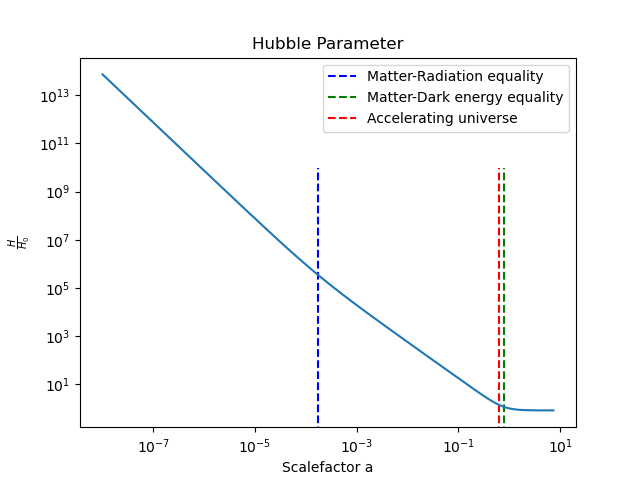
\includegraphics[width=77mm]{Hubble Parameter.png}
	\caption{The evolution of the Hubble parameter.}
	\label{fig:H(x)}
\end{figure}
We see in figure \eqref{fig:H(x)} that the Hubble parameter decreases most of the time. If we start by looking at the period where radiation where the dominant density we can see that the Hubble parameter decreases the most, this makes sense as we look at equation \eqref{eq:Friedmann_eq}, and see that $H\propto \frac{1}{a^2}$. As time passes and we move into the period where matter was the dominant density we see that the Hubble parameter still decreases, but not as sharp as in the radiation period, the reason for this is that $H\propto \frac{1}{\sqrt{a^3}}$.
When we go towards our present time we see an era where the dominant density in out Universe is dark energy. We know that $H\propto 1$ in the dark energy dominant era, hence we see that the Hubble parameter stays constant as in figure \eqref{fig:H(x)}. In the plot we can also see that the universe starts to accelerate  right before we meet the Matter-Dark energy equality. 
\begin{figure}[H]
	\centering
	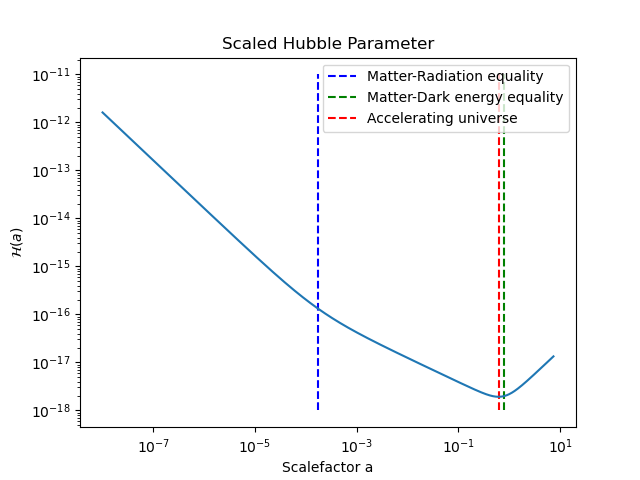
\includegraphics[width=77mm]{Scaled Hubble Parameter.png}
	\caption{The evolution of the scaled Hubble parameter}
	\label{fig:Hp(x)}
\end{figure}
Also in figure \eqref{fig:Hp(x)} we see that scaled Hubble parameter decreases, but this one decreases slower than $H$. This comes from that $\mathcal{H}\propto \frac{1}{a}$ for radiation dominated time, for matter dominated time $\mathcal{H}$ decreases slower than the  radiation dominated time, this comes from that $\mathcal{H}\propto \frac{1}{\sqrt{a}}$. For the dark energy dominated time will $\mathcal{H}$ start to increase, due to $\mathcal{H}\propto {a}$ for dark energy dominated time. \\
\\
In figure \eqref{fig:der_Hp(x)} we see the behaviour of the first and second derivative of $\mathcal{H}$, the most interesting thing about this figure is to see what happens at $\frac{d\mathcal{H}}{dx}=0$. At this point we see that the universe starts to accelerate. By using equation \eqref{eq:H_rho} we found $\frac{d\mathcal{H}}{dx}/H$ and $\frac{d^2\mathcal{H}}{dx^2}/H$
\begin{figure}[H]
	\centering
	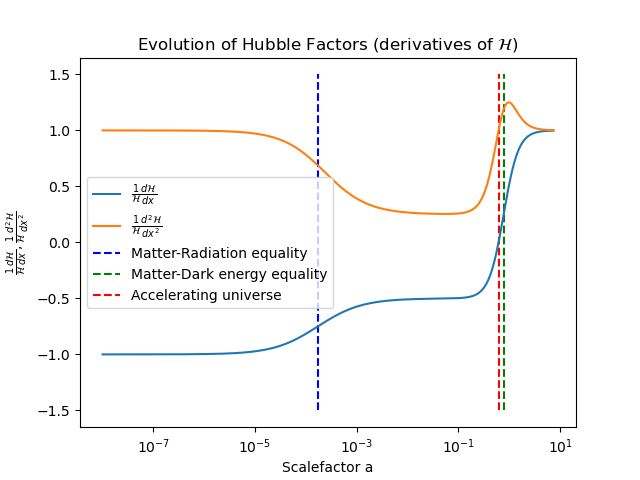
\includegraphics[width=77mm]{der_Hp.png}
	\caption{The behavior of the first and second derivatives of $\mathcal{H}$ as the scalefactor increases.}
	\label{fig:der_Hp(x)}
\end{figure}
\begin{align}
    \frac{d\mathcal{H}(x)}{dx}/H&=-\frac{1}{2}(1+3\omega) \label{eq:der_H_om}\\
    \frac{d^2\mathcal{H}(x)}{dx^2}/H&=\frac{1}{4}(1+3\omega)^2 \label{eq:der_H2_om}
\end{align}
See appendix \eqref{A.1} for the calculation.\\
If we now insert equation \eqref{eq:omega_val} into \eqref{eq:der_H_om} and \eqref{eq:der_H2_om} we get
\begin{align}
\frac{d\mathcal{H}(x)}{dx}/H&=
  -\frac{1}{2}\;\; \text{for cold dark matter and baryons}\notag\\
  &=-1\;\; \text{for radiation}\notag\\
  &=1\;\; \text{for dark energy}
 \label{eq:derH_inserted}
\end{align}
\begin{align}
\frac{d^2\mathcal{H}(x)}{dx^2}/H&=
  \frac{1}{4}\text{for cold dark matter and baryons}\notag\\
  &=1\text{for radiation}\notag\\
    &=1 \text{for dark energy}  \label{eq:derH2_inserted}
\end{align}
So if we look at equation \eqref{eq:derH_inserted} we see that $\frac{d\mathcal{H}(x)}{dx}/H$ should be at $-1$ for the radiation dominated time, and as it moves to the matter-dominated time it should be $-\frac{1}{2}$ and $1$ at the dark energy-dominated time. So these values indicates that the $\frac{d\mathcal{H}(x)}{dx}/H$ plot looks right. For the $\frac{d^2\mathcal{H}(x)}{dx^2}/H$ we found that it should be $1$ for radion-dominated time, $\frac{1}{4}$ for matter-dominated time and $1$ for dark energy-dominated time as we can see in equation \eqref{eq:derH2_inserted}. These values also fits our plot for $\frac{d^2\mathcal{H}(x)}{dx^2}/H$.  
\begin{figure}[H]
	\centering
	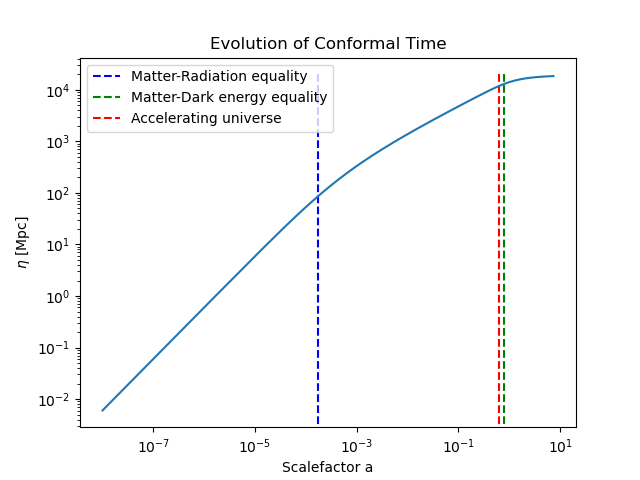
\includegraphics[width=77mm]{Evolution of Conformal Time.png}
	\caption{The conformal time $\eta$. Shows the evolution of the universe}
	\label{fig:Ev_Conf_time(x)}
\end{figure}
\begin{figure}[H]
	\centering
	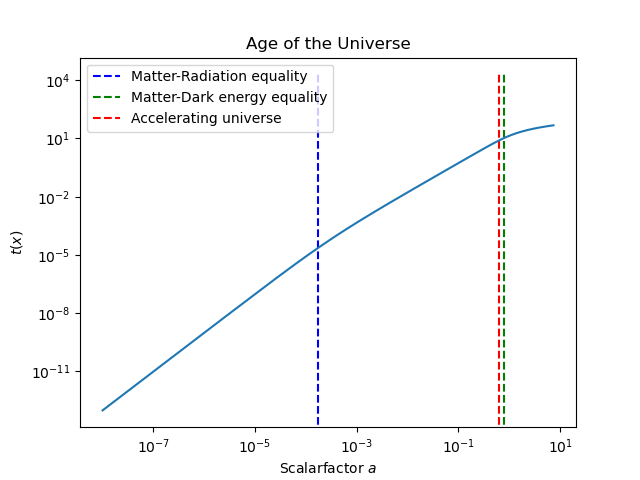
\includegraphics[width=77mm]{t_of_x.png}
	\caption{The age of the universe as a function of the scalefactor}
	\label{fig:t_of_x}
\end{figure}
We now that $\eta \propto a$ in the radiation dominated time. This indicates that figure \eqref{fig:Ev_Conf_time(x)} looks right since $\eta$ is moving linear with the scalar factor in the radiation dominated time. For the matter dominated time we have that $\eta\propto \sqrt{a}$. And our figure here also looks right since $\eta$ still increases as we move in the matter dominated time, but not as sharply when radiation was the dominant density. In the dark energy dominated time will $\eta \propto 1$, hence will $\eta$ move constant horizontal as in figure \eqref{fig:Ev_Conf_time(x)}. And we find that the Conformal time today is 
\begin{align}
    \eta(0)=46.25\text{Gyr}
\end{align}
We see in figure \eqref{fig:t_of_x} that when we reach the time where  dark energy is the dominated density, that the universe does not expand constant anymore. The expansion is now accelerating! We also find the age of the universe today, which is
\begin{align}
    t(0)=13.77 \text{Gyr}
\end{align}
which is a reasonable number.
\begin{figure}[H]
	\centering
	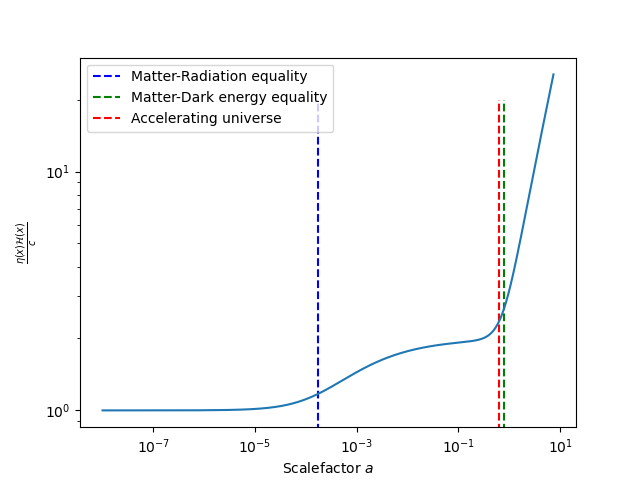
\includegraphics[width=77mm]{eta_Hp_c.png}
	\caption{Checking the values of $\eta$ and $\mathcal{H}$}
	\label{eq:eta_Hp_c}
\end{figure}
Figure \eqref{eq:eta_Hp_c} is just a test to see if the values for $\eta$ and $\mathcal{H}$ is correct. If we look at the radiation dominated time we have that $\eta=a$ and $\mathcal{H}=\frac{1}{a}$. This means that $\eta\mathcal{H}=a\frac{1}{a}=1$ which fits for our figure where radiation was the dominant density. 
\begin{figure}[H]
	\centering
	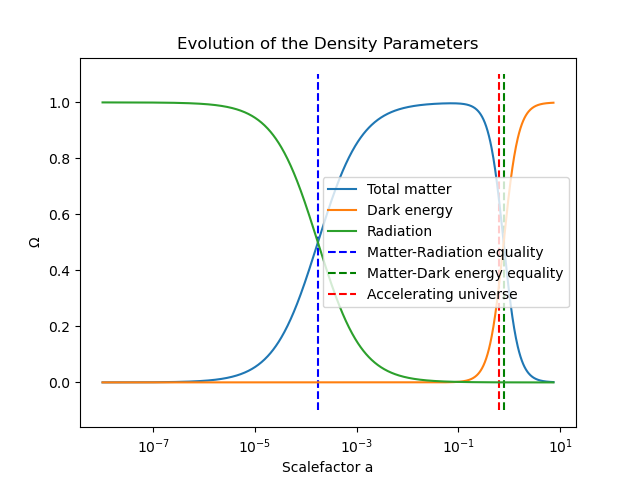
\includegraphics[width=77mm]{Omega.png}
	\caption{Evolution of the density parameters}
	\label{fig:Omega}
\end{figure}
In figure \eqref{fig:Omega} we can see that the evolution of the density parameters. We see that at the beginning the radiation density was the fully dominated density. As the scalefactor increases, the matter density increases as well and gets fully dominant for a period. As we goes towards our time the universe starts to accelerate and the dark energy density gets equal to the matter density, after the scalefactor increases more we see that the dark energy density dominates the universe right now. \\
\begin{figure}[H]
	\centering
	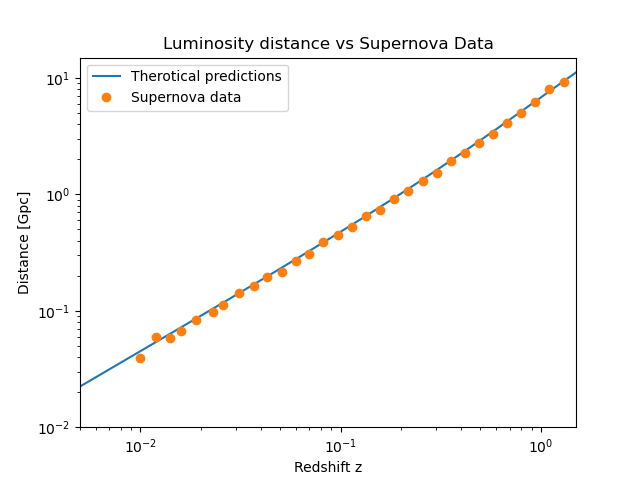
\includegraphics[width=77mm]{LD_vs_SN.png}
	\caption{Theoretical predictions of the luminosity distance compared with supernova data.}
	\label{fig:LD_vs_SN}
\end{figure}
We see that our theoretical predictions fits well with the data we received from the supernova, which makes sense since the errors we got where small.
\clearpage
\section{Milestone 2}
\subsection{Introduction}
In this project we are going to look at the recombination history of the universe. More detailed, we will investigate how baryons went from being ionized to neutral. Further we will calculate the optical depth, $\tau$, and it's derivatives, as well as the the visibility function, $\Tilde{g}$, and it's derivatives. 
\subsection{Theoretical Background}
The definition of recombination is that the universe goes from being tightly coupled plasma of electrons and protons, to electrons and protons binding together and creating hydrogen. This can be done when the temperature of the primordial plasma gets smaller than the binding energy. Due to recombination we will get cosmic microwave background since the photons can move freely with scattering free electrons.
\subsubsection{Boltzmann Equation}
The Boltzmann equation can be used to describe all kind of interactions. It can for example be used to describe how electrons and protons interact and creates hydrogen. And vice versa, where photons ionize hydrogen, which gives us a free electron and free proton
\begin{align*}
    e^- + p^+ \rightleftharpoons H + \gamma
\end{align*}
where $e^-$ is the electron, $p^+$ is the proton, $H$ is the hydrogen and $\gamma$ is the photon.\\
If we consider a smooth universe we can write the Boltzmann equation on the following form
\begin{align}
    \frac{1}{a^3}\frac{d(n_1 a^3)}{dt} = -\alpha n_1n_2 + \beta n_3n_4 \label{eq:BE}
\end{align}
where $a$ is the scalarfactor, $n_i$ is the number density, $\alpha = \left<\sigma v\right>$ is the thermally averaged cross-section and $\beta$ is the full derivation from the collision term. By equilibrium we can cancel the left hand side and the right hand side of equation \eqref{eq:BE}, hence $n_i$ possess the equilibrium value
\begin{align}
    \beta &= \alpha \left(\frac{n_1n_2}{n_3n_4}\right)_{\rm eq} \notag\\
    \frac{1}{a^3}\frac{d(n_1 a^3)}{dt} &= -\left<\sigma v\right>  \left(n_1n_2 - n_3 n_4 \left(\frac{n_1n_2}{n_3n_4}\right)_{\rm eq}\right) \label{eq:H_pro}
\end{align}
which we rewrite as
\begin{align}
    \frac{1}{n_1a^3}\frac{d(n_1 a^3)}{d x} = - \frac{\Gamma_1}{H}\left(1 - \frac{n_3 n_4}{n_1n_2} \left(\frac{n_1n_2}{n_3n_4}\right)_{\rm eq}\right) \label{eq:RW2_BE}
\end{align}
where $H$ is the expansion rate and $\Gamma_1 \equiv n_2\left<\sigma v\right>$ is the interaction rate. The second part on the right hand side of equation \eqref{eq:RW2_BE} tells us how far away we are to reach equilibrium, as well as it gives us information about decoupling and freeze-out.\\
To reach chemical equilibrium we must have that $\Gamma_1 \gg H$, which means that the interaction rate is greater than the expansion rate of the universe. This means that we get a lot of interactions while the universes size doubles. Hence we will keep equilibrium. It is important to remember that we have the relation $n_i^{\rm eq} \propto e^{-\frac{m}{T}}$, hence the equilibrium distribution decreases exponentially as the temperature decreases. If we now consider that $\Gamma_1 < H$ will there be no equilibrium since the efficiency of interaction is to small which leads to decoupling. For $\Gamma_1 \ll H$ will there be no interaction, and we get volume dilution in an expanding universe, $n_1\propto 1/a^3$. This is due to that equation \eqref{eq:RW2_BE} will be zero, $\frac{d(n_1a^3)}{dx}\approx0$. This is known as freeze-out for massive particles.
\subsubsection{Saha Approximation}
The Boltzmann equation \eqref{eq:RW2_BE} can be written as
\begin{align}
    \left(1 - \frac{n_3 n_4}{n_1n_2} \left(\frac{n_1n_2}{n_3n_4}\right)_{\rm eq}\right) &\approx 0 \notag\\
    \frac{n_1n_2}{n_3n_4} &\approx \left(\frac{n_1n_2}{n_3n_4}\right)_{\rm eq} \label{eq:Saha_approx}
\end{align}
when the efficiency of interaction is high enough to get close to equilibrium. This equation is also known as the Saha approximation. \\
We can rewrite equation \eqref{eq:Saha_approx}. We know that the universe is electrically neutral, hence $n_e=n_p$. Further we have that $n_\gamma = n_\gamma^{\rm eq}$ since photons are in equilibrium with primodial plasma. Furthermore by only considering hydrogen as the number density for baryon $n_b \approx \frac{\rho_b}{m_H}$, where $\rho_b = \rho_{c0}\frac{\Omega_{b0}}{a^3}$, $m_H$ is the hydrogen mass and $\rho_{c0} = \frac{3H_0^2}{8\pi G}$. At last we have that the free electron fraction is given as $X_e = \frac{n_e}{n_b}$, where $n_b \approx n_p + n_H = n_e + n_H$. We now have the information needed for the Saha equation which is defined as 
\begin{align}
    n_b\frac{X_e^2}{(1 - X_e)} = \left(\frac{n_en_p}{n_H}\right)_{\rm eq} \label{eq:Saha_eq}
\end{align}
where
\begin{align*}
    \left(\frac{n_en_p}{n_H}\right)_{\rm eq} = \left(\frac{T m_em_p}{2\pi m_H}\right)^{3/2} e^{-\frac{m_e + m_p - m_H}{T}}
\end{align*}
where $\epsilon_0=\frac{m_e + m_p - m_H}{T}\approx13.6\text{eV}$ is the binding energy of hydrogen and $\frac{m_p}{m_e}\approx1$. The Saha equation is now defined as
\begin{align}
    \frac{X_e^2}{(1 - X_e)} = \frac{1}{n_b}\left(\frac{k_bT m_e}{2\pi \hbar^2}\right)^{3/2} e^{-\frac{\epsilon_0}{k_bT}} \label{eq:Saha_2}
\end{align}
where $c$, $\hbar$ and $k_b$ is the speed of light, reduced Planck constamt and Boltzmann constant respectively. 
\subsubsection{Peebles Equation}
The Saha approximation for the Boltzmann equation is only valid when $X_e\approx1$, so when it increases or decreases it is not valid anymore. Another way to solve the Boltzmann equation is to use Peebles equation.  \\
By using the definition of electron fraction, $n_\gamma = n_\gamma^{\rm eq}$ and $n_e=n_p$ as we used for the Saha approximation and insert those into equation \eqref{eq:H_pro} we get \begin{align}
    \frac{dX_e}{dx} = \frac{1}{H}  \left((1 - X_e) \beta - n_b \alpha^{(2)} X_e^2\right)
\end{align}
where $\alpha^{(2)} = \left<\sigma v\right>$ and $\beta = \left<\sigma v\right>\left(\frac{k_bT m_em_p}{2\pi m_H}\right)^{3/2} e^{-\frac{m_e + m_p - m_H}{k_bT}}$\\
The downside with the Peebles equation is that the electron in a hydrogen atom can have different energy and spin states. To recombine a hydrogen atom to its ground state requires that a photon is emitted with a energy greater than the ground state of a hydrogen atom, $13.6$ eV. When this is done will the photon probably ionize another atom. Hence the the total effect will be $\sim0$. So electrons is only effectively recombined to the excited states of hydrogen, where they go off to the first excited state with quantum number $n=2$. There are now two possible ways to reach the ground state. The first one is that an emitted photons frequency decreases due to cosmological redshift. Due to this the escape of the reabsorption of a photon hitting another hydrogen atom gets smaller if its frequency is redshifted enough before hitting the hydrogen atom. The second option is to emit two photons from the $2s$ state. The rate of this process is $\Lambda_{2s\to 1s} = 8.22 s^{-1}$ and is very slow. So it is possible that the atoms is getting reionized in the first excited state before it gets to the ground state.\\
So from these two possible ways there is introduced a factor which looks at the probability of an atom to reach it ground state from the first excited state, it is defined as $C_r$. And the Peebles equation is now defined as 
\begin{align}
    \frac{dX_e}{dx} = \frac{C_r(T_b)}{H} \left[\beta(T_b)(1-X_e) - n_H
\alpha^{(2)}(T_b)X_e^2\right] \label{eq:Peebles_eq_Cr}
\end{align}
where $T_b$ is the baryon temperature and 
\begin{align*}
C_r(T_b) &= \frac{\Lambda_{2s\rightarrow1s} +
\Lambda_{\alpha}}{\Lambda_{2s\rightarrow1s} + \Lambda_{\alpha} +
\beta^{(2)}(T_b)}\\
\Lambda_{2s\rightarrow1s} &= 8.227 \textrm{s}^{-1},\\
\Lambda_{\alpha} &= H\frac{(3\epsilon_0)^3}{(8\pi)^2 c^3\hbar^3 n_{1s}}\\
n_{1s} &= (1-X_e)n_H\\
n_H &= (1-Y_p)n_b\\
n_b &= (1-Y_p)\frac{3H_0^2 \Omega_{b0}}{8\pi G m_H a^3}\\
\beta^{(2)}(T_b) &= \beta(T_b) e^{\frac{3\epsilon_0}{4k_bT_b}}\\
\beta(T_b) &= \alpha^{(2)}(T_b) \left(\frac{m_e k_b
T_b}{2\pi \hbar^2}\right)^{3/2} e^{-\frac{\epsilon_0}{k_bT_b}}\\
\alpha^{(2)}(T_b) &= \frac{8}{\sqrt{3\pi}}
c\sigma_T\sqrt{\frac{\epsilon_0}{k_bT_b}}\phi_2(T_b)\\
\phi_2(T_b) &= 0.448\ln\left(\frac{\epsilon_0}{k_bT_b}\right)
\end{align*}
\subsubsection{Optical Depth}
Optical depth, $\tau$, describes the level of transparency through a medium. An appropriate way to describe the optical depth is to evaluate the intensity of a source which is given as 
\begin{align*}
    I(r)=I_0e^{-\tau(r)}
\end{align*}
where $I_0$ is the intensity of the emiting source. We see that for large $\tau \gg1$ will $I$ get small, hence the medium is optically thick. For small optical depths, $\tau\ll1$, will the intensity stay large, hence the medium is optically thin. At $\tau\sim 1$ we have something called Thompson scattering of photons of free electrons, which is the main absorption in cosmology. This optical depth evaluate the probability for scattering of a photon between an earlier time until this day, and it is given as
\begin{align}
    \tau(\eta)=\int_\eta^{\eta_0}n_e\sigma_Tad\eta\label{eq:Thompson_optical}
\end{align}
where $n_e=n_e(\eta)$ is the electron density, $\eta$ is the time, $\sigma_T=\frac{8\pi}{3}\frac{\alpha^2\hbar^2}{m_e^2c^2}$ is the Thompson cross-section and $a$ is the scalefactor. \\
It can also be looked at the number of scatterings of photons by electrons per unit time.  \\
At the recombination time where the free protons and the free electrons ties together and create hydrogen is also the time when the universe has its passage from being optically thick to optically thin.
\subsubsection{Visibility function}
The visibility function is a probability distribution which describes the probability density for a photon to last time having scattered at time x, and its defined as
\begin{align}
    \tilde g(x) = -\tau' e^{-\tau}=-\frac{d\tau}{dx}e^{-\tau}\\
    \int_\infty^0\tilde g(x)dx=1
\end{align}
\subsection{Method}
We will solve the recombination history of the universe numerically. To do so we first start to solve the Saha equation to calculate $X_e$ and $n_e$, this equation is only valid until $X_e\sim 0.99$. After that we switch to the Peebles equation. We solve the Peebles equation by using Runge-Kutta 4 method to solve $X_e$ and use a qubic spline on $X_e$ and $n_e$.\\
With $n_e$ we are able to calculate the optical depth. We use the Runge-Kutta 4 method and spline the solution. We do the same thing for $\frac{d\tau}{dx}$. For $\frac{d^2\tau}{dx^2}$ we use a '$\text{deriv}_x$'-function.\\
For the visibility function $\tilde g$ we use the Runge-Kutta 4 ODE solver and spline the solution and  use a '$\text{deriv}_x$'-function on $\frac{d\tilde g}{dx}$ and $\frac{d^2\tilde g}{dx^2}$\\
The calculation on the decoupling and recombination on $x$ is to use 'binary search for value'-function and set $\tau=1$ for decoupling and $X_e=0.5$ for recombination. For the redshift we just say $z=1/e^{x}-1$. 
\subsection{Results}
We used $\tau=1$ for finding the time for the last scattering surface 
\begin{align*}
    x_\text{decoupling} &=-6.98\\
    z_\text{decoupling}&=1081.15
\end{align*}
Further we found the time when the recombination was half-way at $X_e=0.5$
\begin{align*}
    x_\text{rec} &=-7.16\\
    z_\text{rec}&=1291.25
\end{align*}
Then we found the freeze-out abudance of free electrons
\begin{align*}
    X_e(x=0)=0.000197
\end{align*}
\begin{figure}[H]
	\centering
	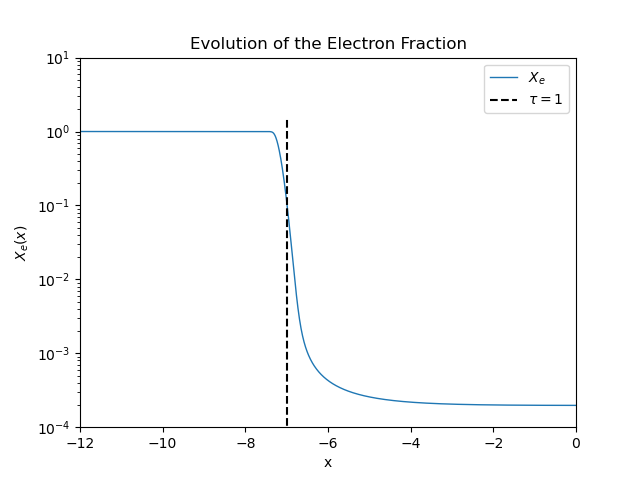
\includegraphics[width=77mm]{Electron_fraction.png}
	\caption{Fractional electron density, $X_e$ as a function of time $x$. }
	\label{fig:X_e}
\end{figure}
If we consider that we are in the early universe the temperature will be large. And by looking at the Saha equation \eqref{eq:Saha_eq} will the temperature lead to proportionality $\propto T^{3/2}$ meaning that the right and side will be large. This means we should have that $1-X_e\approx0$, hence $X_e\approx1$ which fits figure \eqref{fig:X_e} in the early universe. If we look at it physically we have large temperature, and large density in the early universe. The temperature will be greater than $\epsilon_0\approx13.6\text{eV}$ at this stage, which means that the photons will have high enough energy to ionize the hydrogen atoms that has been made. By considering a universe with low temperature, $e^{-\frac{\epsilon_0}{k_bT}}\ll1$, hence $X_e\ll1$. Low temperature also means that most of the photons has to low energy to ionize hydrogen atom, so almost all interaction will go $e^- + p^+ \to H +  \gamma$.\\
\begin{figure}[H]
  \resizebox{\hsize}{!}{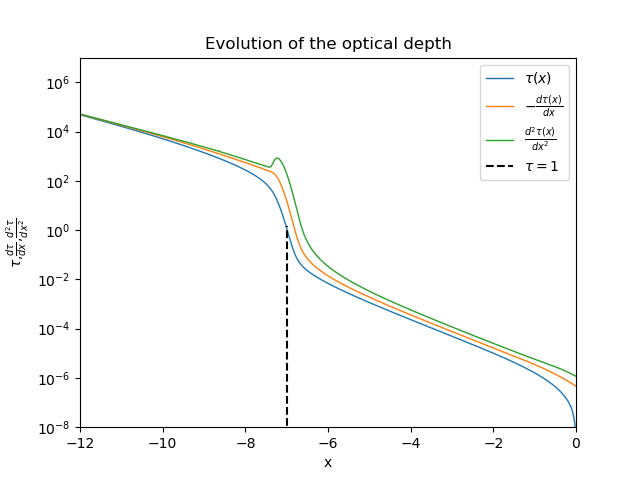
\includegraphics{Optical Depth.png}}
  \caption{Optical depth $\tau$, $\frac{d\tau}{dx}$, $\frac{d^2\tau}{dx^2}$ as a function of time $x$.}
  \label{fig:Otical_depth}
\end{figure}
Figure \eqref{fig:Otical_depth} shows us the behaviour of the optical depth. We see that the optical depth is large at the beginning. When the number of free elctrons falls at $x_\text{decoupling}$ the optical depth decreases fast. \\
\begin{figure}[H]
  \resizebox{\hsize}{!}{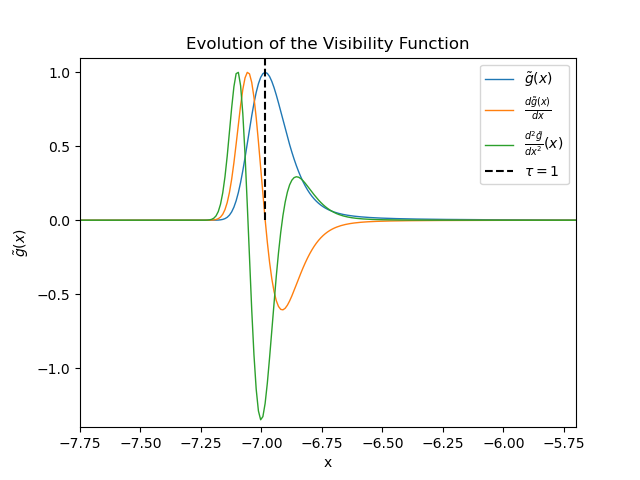
\includegraphics{Visibility_function.png}}
  \caption{Visibility function $\Tilde{g}$, $\frac{d\Tilde{g}}{dx}$ $\frac{d^2\tildeg}{dx^2}$ as a function of time $x$. Where $\Tilde{g}$ is scaled with $(\Tilde{g})_{max}=4.85$,  $\bigg(\frac{d\Tilde{g}}{dx}\bigg)_{max}=50.40$,  $\bigg(\frac{d^2\Tilde{g}}{dx^2}\bigg)_{max}=724.94$}
  \label{fig:Visibility function}
\end{figure}
With less free electrons will photons be able to travel without interact with them as often. Hence we have that the peak of $\tildeg$ is located at $x_\text{decoupling}=-6.98$. This indicates that the that the CMB photons we observe today is scattered around this time. So at $x<x_\text{decoupling}$ will the free electron number be low, so the probability that CMB photons scatter with free electrons is less likely. This means that the visibility function should decrease fast to zero after $x_\text{decoupling}$, which plot \eqref{fig:Visibility function} also do. A sanity check for the visibility function is to look at when $\frac{d\Tilde{g}}{dx}=0$. At $\frac{d\Tilde{g}}{dx}=0$ we should have a maximum point for $\Tilde{g}$, which figure \eqref{fig:Visibility function} has. As well when $\frac{d^2\Tilde{g}}{dx^2}=0$ we should have a maximum point for $\frac{d\Tilde{g}}{dx}$ which our plot also indicates.   
\subsection{Discussion}
We wanted to find where the recombination time $x_\text{rec}$ and $z_\text{rec}$ was when we only used the Saha equation. This gave us the values 
\begin{align*}
    x_\text{rec} &=-7.37\\
    z_\text{rec}&=1590.51
\end{align*}
This is earlier than when we looked at the recombination half-way $X_e=0.5$. 
\begin{figure}[H]
  \resizebox{\hsize}{!}{\includegraphics{bau_rec.png}}
  \caption{Figure taken from Baumann. The evolution of the free electron from the early Universe till today.}
  \label{fig:Bau_rec}
\end{figure}
As mentioned earlier we said that the Saha equation is only valid at $X_e\sim1$. So when $X_e$ is moving away from 1 the Saha approximation fails. We got $x_\text{rec} =-7.37$ and 
    $z_\text{rec}=1590.51$ when we used the Saha approximation, which is earlier than the recombination. By looking at figure \eqref{fig:Bau_rec} we see that as we move away from $X_e\approx1$ the Saha approximation gives us values that is incorrect, and the recombination happens before it should. Hence we can conclude that the Saha approximation is only valid at $X_e\approx1$. \\
    I would like to add a comment that the recombination should be later than the value we got. It should have been close to $x_\text{rec} \sim-7.2$ and $z_\text{rec} \sim1400$ which we can see in figure \eqref{fig:Bau_rec}.   
\clearpage
\section{Milestone 3}
\subsection{Introduction}
In the previous milestones we have considered a smooth Universe(?). We will now take it a step further and use the cosmological perturbation theory to study the evolution of the Universe. To do so we add perturbation to the Einstein and Boltzmann equations. After adding perturbation, we will calculate their evolution in Fourier space. 
\subsection{Theory}
The Boltzmann equation describes the distribution function evolution of some particle species as a function of time, and it is defined as
\begin{align}
    \frac{df}{d\lambda} = C(f) \label{eq:BE_C}
\end{align}
where $C$ gives us information on the interactions and its known as the collision term, and $\lambda$ is an affine parameter.   
To study the evolution of structures in the Universe we have to add perturbations to the distribution function for each species $f_i$ and for our metric. The distribution function with perturbation is given as
\begin{align}
    f_i(t,\vec{x},\vec{p}) = \overline{f_i}(t,\vec{p}) + \delta f_i(t,\vec{x},\vec{p}) \label{eq:pert_f_i}
\end{align}
where $\delta f_i(t,\vec{x},\vec{p})$ is the perturbation term. \\
We will use a Newtonian gauge for our metric which is defined as
\begin{align}
    \mathrm{d} s^{2}= -dt^2(1+2\Psi) + a^2(1+2\Phi)(dx^2 + dy^2 + dz^2) \label{eq:NG}
\end{align}
where $\Psi$ and $\Phi$ are perturbation functions of space and time. Where $\Psi$ corresponds to the Newtonian potential and $\Phi$ corresponds to curvature in space. 
\\
The perturbations to the distribution function is defined as
\begin{align*}
    T = \overline{T}(1 + \Theta(t,\vec{x},p,\hat{p}))
\end{align*}
and it is also known as the perturbation in the local photon temperature
\begin{align}
    \Theta(t,\vec{x},\hat{p}) = \frac{\delta T}{T}
\end{align}
Since the relevant interaction is Compton scattering for photons, it is only the direction of the photon that changes and not the momentum. Hence $\Theta$ only depends on the momentum direction $\hat{p}$ and not the momentum $p$. Compton scattering is scattering of light by free electrons. 
\begin{align*}
    e^- + \gamma \rightleftharpoons e^- + \gamma\\
    p^+ + \gamma \leftrightharpoons p^+ + \gamma
\end{align*}
And the collision term of this process for first order in perturbation theory is given as
\begin{align}
    C = -p^2\frac{\partial \overline{f}}{\partial p}n_e \sigma_T[\Theta_0 - \Theta + \hat{p}\cdot \vec{v}_b]
\end{align}
where $n_e$ is the electron density, $\sigma_T$ is the Thompson cross-section, $\Theta_0 \equiv \frac{1}{4\pi}\int d\Omega_{\hat{p}} \Theta = \frac{1}{2}\int_{-1}^1 \Theta d\mu$ is the monopole moment of the photon distribution and $\Vec{v}_b$ is the baryon velocity. And inserting this into equation \eqref{eq:BE_C} we get 
\begin{align}
    \frac{\partial \Theta}{\partial t} + \frac{\partial \Theta}{\partial x^i} \frac{\hat{p}^i}{a} + (\frac{\partial \Phi}{\partial t} + \frac{\partial \Psi}{\partial x^i}\frac{\hat{p}^i}{a}) = n_e \sigma_T[\Theta_0 - \Theta + \hat{p}\cdot \vec{v}_b] \label{eq:final_photon}
\end{align}
see Appendix B.
Equation \eqref{eq:final_photon} show us that the Compton scattering is efficient, and therefore will the photon distribution get reduced to $\Theta \approx \Theta_0$, which means that at any place in space the photons from different directions will have the selfsame temperature. \\
The Thompson cross-section, $p^+ + \gamma \rightleftharpoons p^+ + \gamma$, has the proportionality $\propto1/m^2$. Since the protons has a much larger mass than the electrons will that process be irrelevant compared to the Compton scattering. In Photon-Photon scattering, $\gamma + \gamma \rightleftharpoons \gamma + \gamma$, will the energy and momentum be conserved, hence this interaction is also irrelevant.  \\
\\
Finally we are able to find all of the Boltzmann equations we need as well as the potential $\Psi$ and $\Phi$ from the Einstein equations. We used the perturbed distribution function from equation \eqref{eq:pert_f_i} to solve the Boltzmann equations, equation \eqref{eq:BE_C}, for all the particle species. With this information we can find the pertubed energy momentum tensor $\delta T_{\mu\nu}$, which will give us the perturbed Einstein equation. The perturbed Einstein equation, $\delta G_{\mu\nu}=8\pi G\delta T_{\mu\nu}$ will give us the metric potentials, $\Phi$, as a Poisson equation, and $\Psi$, it is nice to mention that we are assuming small anisotropic stress. \\
\\
We can use a Fourier transform on equation \eqref{eq:final_photon} to reduce the number of free variables. We start by introducing the $\mu \equiv \frac{\hat{p}\cdot \vec{k}}{k}$-variable, this is the $\cos$-angle between the $\hat{p}$ and the wavevector $\vec{k}$. The baryon velocity is curl-free, hence $\vec{v_b} = iv_b \frac{\vec{k}}{k}$ in the Fourier space. With this information equation \eqref{eq:final_photon} can be written as
\begin{align}
    \frac{\partial \Theta}{\partial t} + \frac{ik\mu}{a} \Theta + (\frac{\partial \Phi}{\partial t} + \frac{i k\mu}{a}\Psi) = n_e \sigma_T[\Theta_0 - \Theta + i\mu v_b - \frac{3\mu^2-1}{4}\Pi] 
\end{align}
where $\Pi = \Theta_2 = -\frac{1}{2}\int_{-1}^1\Theta \frac{3\mu^2-1}{2}d\mu$ is due to the angular dependence of the Compton scattering.\\
We can now write the Einstein-Boltzmann equations which describes the velocity and energy contents as well as the the metric perturbation in Fourier space.
The mertric perturbation 
\begin{align}
\Phi^\prime &= \Psi - \frac{c^2k^2}{3\mathcal{H}^2} \Phi + \frac{H_0^2}{2\mathcal{H}^2}
\left[\Omega_{\rm CDM 0} a^{-1} \delta_{\rm CDM} + \Omega_{b 0} a^{-1} \delta_b + 4\Omega_{\gamma 0}
a^{-2}\Theta_0 \right] \\
\Psi &= -\Phi - \frac{12H_0^2}{c^2k^2a^2}\left[\Omega_{\gamma 0}\Theta_2\right]
\end{align}
The initial conditions  photon temperature multipoles 
\begin{align}
\Theta^\prime_0 &= -\frac{ck}{\mathcal{H}} \Theta_1 - \Phi^\prime, \\
\Theta^\prime_1 &=  \frac{ck}{3\mathcal{H}} \Theta_0 - \frac{2ck}{3\mathcal{H}}\Theta_2 +
\frac{ck}{3\mathcal{H}}\Psi + \tau^\prime\left[\Theta_1 + \frac{1}{3}v_b\right], \\
\Theta^\prime_\ell &= \frac{\ell ck}{(2\ell+1)\mathcal{H}}\Theta_{\ell-1} - \frac{(\ell+1)ck}{(2\ell+1)\mathcal{H}}
\Theta_{\ell+1} \notag \\
&+ \tau^\prime\left[\Theta_\ell - \frac{1}{10}\Pi
\delta_{\ell,2}\right], \quad\quad 2 \le \ell \lt \ell_{\textrm{max}} \\
\Theta_{\ell}^\prime &= \frac{ck}{\mathcal{H}}
\Theta_{\ell-1}-c\frac{\ell+1}{\mathcal{H}\eta(x)}\Theta_\ell+\tau^\prime\Theta_\ell,
\quad\quad \ell = \ell_{\textrm{max}}
\end{align}
The initial condition for CDM and baryons
\begin{align}
\delta_{\rm CDM}^\prime &= \frac{ck}{\mathcal{H}} v_{\rm CDM} - 3\Phi^\prime \\
v_{\rm CDM}^\prime &= -v_{\rm CDM} -\frac{ck}{\mathcal{H}} \Psi \\
\delta_b^\prime &= \frac{ck}{\mathcal{H}}v_b -3\Phi^\prime \\
v_b^\prime &= -v_b - \frac{ck}{\mathcal{H}}\Psi + \tau^\prime R(3\Theta_1 + v_b) 
\end{align}
HVA DE ER, SE W\\
\\
And the initial conditions are given as following
\begin{align*}
\Psi &= -\frac{1}{\frac{3}{2} + \frac{2f_\nu}{5}}\\
\Phi &= -(1+\frac{2f_\nu}{5})\Psi \\
\delta_{\rm CDM} &= \delta_b = -\frac{3}{2} \Psi \\
v_{\rm CDM} &= v_b = -\frac{ck}{2\mathcal{H}} \Psi\\
&\text{Photons:}\\
\Theta_0 &= -\frac{1}{2} \Psi \\
\Theta_1 &= +\frac{ck}{6\mathcal{H}}\Psi \\
\Theta_2 &= \left\{
\begin{array}{l}
-\frac{8ck}{15\mathcal{H}\tau^\prime} \Theta_1, \quad\quad \textrm{(with polarization)} \\
-\frac{20ck}{45\mathcal{H}\tau^\prime} \Theta_1, \quad\quad \textrm{(without polarization)}
\end{array}\right. \\
\Theta_\ell &= -\frac{\ell}{2\ell+1} \frac{ck}{\mathcal{H}\tau^\prime} \Theta_{\ell-1}
\end{align*}
We want to expand the $\mu$-dependence of $\Theta$ in Legendre multipoles. The reason why we do this is that we want to get the equation for photon temperature perturbation on a simpler form since it already depends on the  angular integrals $\Theta_0$ and $\Theta_1$. So we say that
\begin{align}
    \Theta(t,k,\mu) = \sum \frac{2\ell + 1}{i^\ell}\Theta_\ell(t,k) P_\ell(\mu)
\end{align}
where $(2\ell+1)/i^\ell$ is a convention, $\Theta_\ell = \frac{i^\ell}{2}\int_{-1}^1 \Theta(t,k,\mu) P_\ell(\mu)d\mu$ are the multipoles of the photon and $P_\ell$ is the Legendre polynomials. 
\\
\\
The optical depth, $\tau$, is very high at early times. Hence electrons is only affected by temperature fluctions of electrons that are close by. This means that our system will be in thermodynamic equilibrium, and therefore will there only be smooth fluctuations. This regime is named tight coupling. In this regime there is only three relevant multipoles. The monopole, $\Theta_0$, the dipole, $\Theta_1$, and the quadruple, $\Theta_2$. $\Theta_0$ measure the mean temperature at the electrons position. $\Theta_1$ is stated by the velocity of the fluid. And $\Theta_2$ is the only applicable source of polarization signals. 
\subsection{Method}
In the tight coupling regime $\tau'$ is going to be very large, this means that we get an factor $(3\Theta_1 + v_b)$ extra in the Boltzmann equations. This factor is small at this regime, meaning that we get a numerical instability. So we have to create a numerical stable equation for $(3\Theta_1 + v_b)$.
\begin{align}
    q &= \bigg[-(\tau^{\prime\prime}(1+R) + (1-R)\tau^\prime)\left[3\Theta_1 + v_b\right] - \frac{ck}{\mathcal{H}}\left(\Psi + \Theta_0' - 2\Theta_2' \notag\\
    &+ (1- \frac{\mathcal{H}^\prime}{\mathcal{H}})(\Theta_0 - 2\Theta_2)\right)\bigg] \;\bigg/\;\bigg[{\tau^\prime(1+R) + \frac{\mathcal{H}^\prime}{\mathcal{H}} - 1}\bigg]
\end{align}
\begin{align}
    v_b^\prime = \frac{1}{1+R} \left[-v_b - \frac{ck}{\mathcal{H}}\Psi + R(q + \frac{ck}{\mathcal{H}}(-\Theta_0 + 2\Theta_2) - \frac{ck}{\mathcal{H}}\Psi)\right]
\end{align}
\begin{align}
    \Theta_1'=\frac{1}{3}(q-v_b') \label{eq:that_approx} 
\end{align}
The derivation can be found in Milestone 3 - Appendix (\eqref{M3}).\\
As we solve the Einstein-Boltzmann equations we have to us the approximation given in equation \eqref{eq:that_approx} and ignoring the multipoles when $l>2$. For the other Einstein-Boltzmann equation we can solve them as normal. We have to consider tight coupling at any time before recombination when 
\begin{align}
    \bigg|\frac{d\tau}{dx}\bigg|<10\cdot \text{max}(1,\frac{ck}{\mathcal{H}}
\end{align}
So we solve the Einstein-Boltzmann equations numerically and at tight coupling we only consider the multipoles $\Theta_l$ when $l\leq$ and use our approximation on $\Theta_1'$. When the tight coupling ended we used the Einstein-Boltzmann equations on the multipoles $\Theta_l$ up to $l<8$. 
\\
\subsection{Results and Discussion}
\begin{figure}[H]
	\centering
	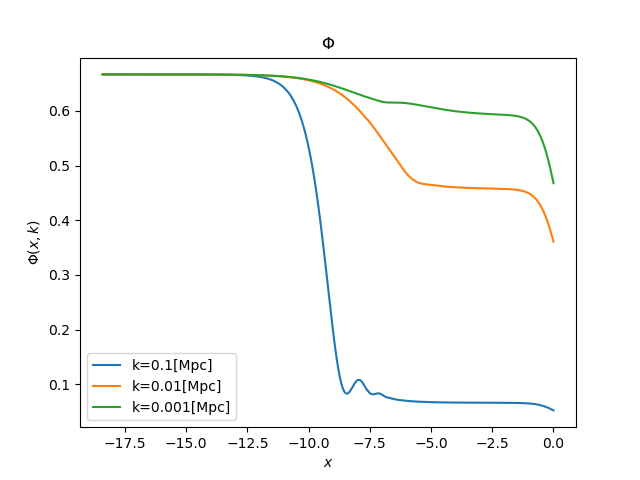
\includegraphics[width=77mm]{phi.png}
	\caption{Evolution of the Newtonian potential $\Phi$.}
	\label{fig:phi}
\end{figure}
\begin{figure}[H]
	\centering
	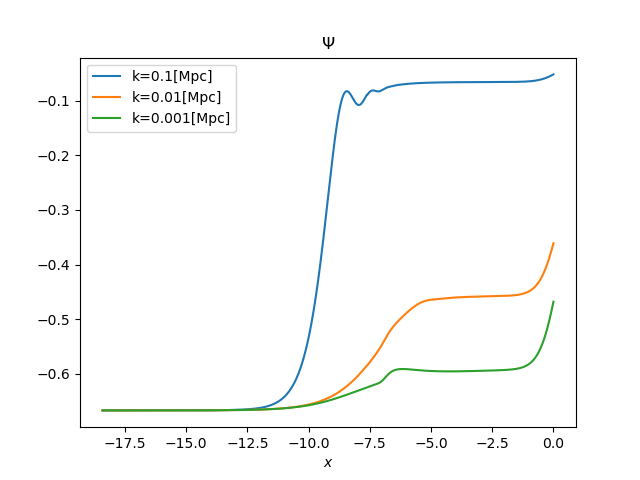
\includegraphics[width=77mm]{psi.png}
	\caption{Evolution of $\Psi$.}
	\label{fig:psi}
\end{figure}
\begin{figure}[H]
	\centering
	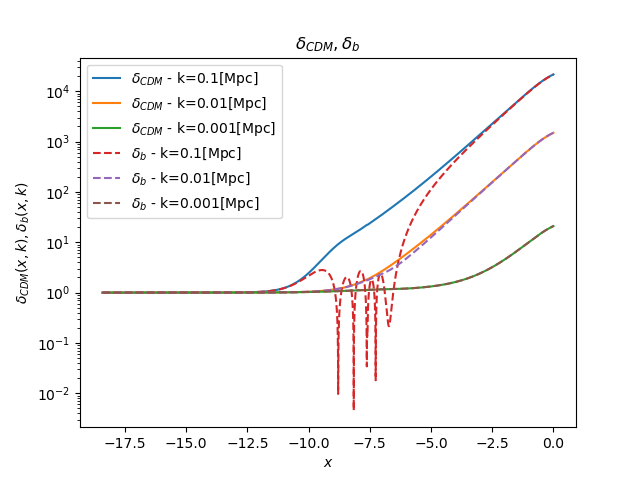
\includegraphics[width=77mm]{delta_.png}
	\caption{The density evolution for cold dark matter $\delta_{CDM}$ and baryon $\delta_b$.}
	\label{fig:delta_}
\end{figure}
\begin{figure}[H]
	\centering
	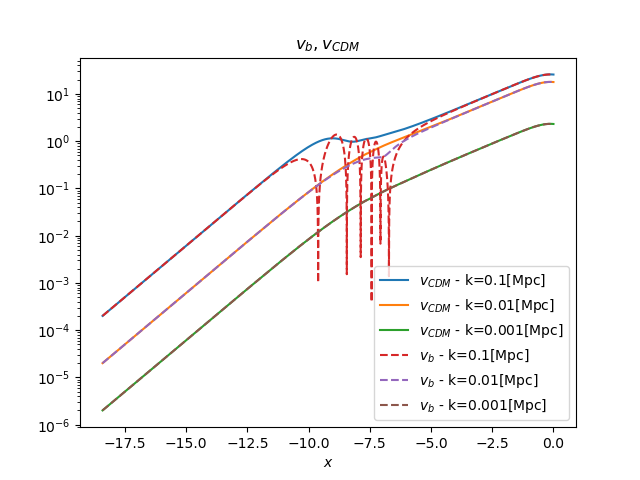
\includegraphics[width=77mm]{v_.png}
	\caption{The velocity perturbation evolution for cold dark matter $\delta_{CDM}$ and baryon $\delta_b$.}
	\label{fig:v_}
\end{figure}
\begin{figure}[H]
	\centering
	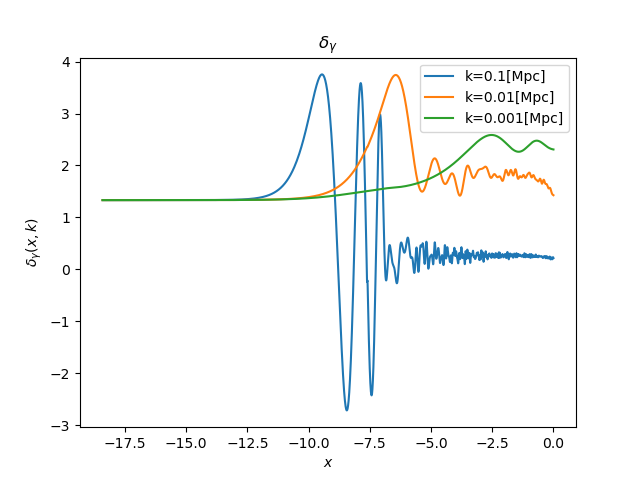
\includegraphics[width=77mm]{delta_gamma.png}
	\caption{The photon density evolution $\delta_\gamma=4\Theta_0$.}
	\label{fig:delta_gamma}
\end{figure}
\begin{figure}[H]
	\centering
	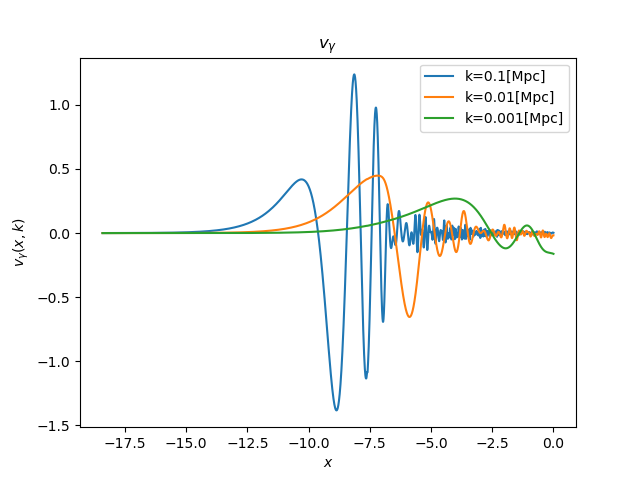
\includegraphics[width=77mm]{v_gamma.png}
	\caption{The photon velocity perturbation evolution $v_\gamma=-3\Theta_1$.}
	\label{fig:v_gamma}
\end{figure}
At the start we have that the mode is frozen outside the horizon at $k\eta\gg1$. Due to this we get that the density contrasts for cold dark matter and baryon has a constant movement at the beginning, which we also can see in figure \eqref{fig:delta_}. When we get closer to the horizon, $k\eta\approx1$, will gravity start to act on the densities contrasts. When the gravity increases the CDM density contrasts also increases. And when the CDM density contrasts reaches the dark energy dominated era the density contrasts settles. This comes from that the universe has already expanded a lot so there will be no more clusters to make. Rikig? HVORFOR GJØR DEN DET? If we look at the density contrasts for baryons we see that low baryon mode, $k=0.1$, causes oscillations, this comes from that this density contrast reaches the horizon before recombination. This means that baryons and photons are still tightly coupled. Hence the fluid of the baryon-photon will create pressure which press the gravity, and therefore creating oscillation. After the recombination the oscillation ends and the low mode density contrast, $k=0.1$, moves to the density contrast for the CDM. \\
We see the same behaviour for the velocity perturbation in figure \eqref{fig:v_}. The low mode velocity perturbation for baryons start to oscillate around the recombination time where the pressure presses against gravity. And after the decoupling will the velocity perturbation for baryon be caught by the gravitation from dark matter. \\
Figure \eqref{fig:phi} shows us the spatial curvature. We see that it has a constant movement until it reaches the horizon. The reason for why this potential falls is due to the dilution of the density in an expanding universe. For $k=0.1$ we get oscillation at the recombination time. DE ERA. \\
In figure \eqref{fig:delta_gamma} and \eqref{fig:v_gamma} we see the photon density contrast and photon velocity perturbation. We see that there are oscillation when we get to the horizon. And when we reach the recombination will the oscillation decay.\\

% WARNING
%----- is not --------------------------------------------------------------
% Please note that we have included the references to the file aa.dem in
% order to compile it, but we ask you to:
%
% - use BibTeX with the regular commands:
%   \bibliographystyle{aa} % style aa.bst
%   \bibliography{Yourfile} % your references Yourfile.bib
%
% - join the .bib files when you upload your source files
%-------------------------------------------------------------------
\clearpage
\appendix % Her kommer appendix.

\subsection{Appendix A}
\label{A.1}
\subsubsection{$\frac{d\mathcal{H}(x)}{dx}/H$ and $\frac{d^2\mathcal{H}(x)}{dx^2}/H$}
\begin{align*}
    {\mathcal{H}}&=e^xH\\
    &=e^xH_0\sqrt{\frac{\rho_x}{\rho_c}}\\
    &=H_0\frac{1}{\sqrt{\rho_c}}e^{-\frac{3}{2}(1+\omega)+x}\\
    &=\frac{H_0}{\sqrt{\rho_c}}e^{-\frac{1}{2}x-\frac{3}{2}(x\omega}\\
    &=H_0\frac{1}{\sqrt{\rho_c}}e^{-\frac{1}{2}x(1+\omega)}\\
\end{align*}
We now use the $\mathcal{H}$ we got to find $\frac{d\mathcal{H}}{dx}$ 
\begin{align*}
    \frac{d\mathcal{H}}{dx}&=\frac{H_0}{\rho_c}\bigg(-\frac{1}{2}(1+3\omega)\bigg)e^{-\frac{1}{2}x}
\end{align*}
Which finally gives us 
\begin{align}
    {\frac{d\mathcal{H}(x)}{dx}/H}&=\frac{\frac{H_0}{\rho_c}\bigg(-\frac{1}{2}(1+3\omega)\bigg)e^{-\frac{1}{2}x}}{\frac{H_0}{\rho_c}e^{-\frac{1}{2}x}}\\
    &=-\frac{1}{2}(1+3\omega)
\end{align}
We will now find $\frac{d^2\mathcal{H}(x)}{dx^2}/H$, and we do this by first finding the derivative of $\frac{d\mathcal{H}(x)}{dx}$
\begin{align}
    \frac{d^2\mathcal{H}(x)}{dx^2}/H=\frac{H_0}{\sqrt{\rho_c}}\frac{1}{4}(1+3\omega)^2e^{-\frac{1}{2}x} 
\end{align}
Which now gives us $\frac{d^2\mathcal{H}(x)}{dx^2}/H$
\begin{align}
    \frac{d^2\mathcal{H}(x)}{dx^2}/H&=\frac{\frac{H_0}{\sqrt{\rho_c}}\frac{1}{4}(1+3\omega)^2e^{-\frac{1}{2}x} }{\frac{H_0}{\rho_c}e^{-\frac{1}{2}x}}\\
    &=\frac{1}{4}(1+\omega)^2
\end{align}
\clearpage
\subsection{Appendix B}
\label{B_A}
\begin{align}
    \frac{df}{d\lambda} &=C(f)\\
    \frac{df}{d\lambda} &= -P^0p\frac{\partial \overline{f}}{\partial p}\left[\frac{\partial \Theta}{\partial t} + \frac{\partial \Theta}{\partial x^i} \frac{\hat{p}^i}{a} + (\frac{\partial \Phi}{\partial t} + \frac{\partial \Psi}{\partial x^i}\frac{\hat{p}^i}{a})\right]\\
    \frac{\partial \Theta}{\partial t} + \frac{\partial \Theta}{\partial x^i} \frac{\hat{p}^i}{a} + (\frac{\partial \Phi}{\partial t} + \frac{\partial \Psi}{\partial x^i}\frac{\hat{p}^i}{a}) = n_e \sigma_T[\Theta_0 - \Theta + \hat{p}\cdot \vec{v}_b]
\end{align}
\clearpage
\begin{thebibliography}{}

  \url{https://cmb.wintherscoming.no/pdfs/baumann.pdf}\\

   \url{https://cmb.wintherscoming.no/milestone2.php#Overview}\\

   \url{https://cmb.wintherscoming.no/theory_thermodynamics.php#}\\
   \url{https://arxiv.org/pdf/astro-ph/0606683.pdf} \label{Callin}\\
   \url{https://cmb.wintherscoming.no/milestone3.php}\label{M3}
\end{thebibliography}

\end{document}